\documentclass[a4paper,12pt]{article}
\usepackage[bahasa]{babel}
\usepackage{graphicx}
\usepackage{multirow}
\usepackage{enumitem}
\usepackage{listings}
\usepackage{adjustbox}
\graphicspath{ {./img/} }
\begin{document}
\title{Laporan Praktikum Statistika Pertemuan 12}
%\author{Aldzikri Dwijayanto Prathama \\ {\small 195410189}}
\author{Aldzikri Dwijayanto Prathama 
	\\195410189}
\makeatletter
\begin{titlepage}
	\begin{center}
		{\huge \bfseries \@title }\\[14ex]
		
\includegraphics[scale=.8]{logo}\\[4ex]
		{\large \@author}\\[20ex]
		{\large \bfseries {SEKOLAH TINGGI MANAJEMEN INFORMATIKA DAN KOMPUTER
				AKAKOM YOGYAKARTA}}
	\end{center}


%{\large \@date} 
\end{titlepage}
\makeatother
%\maketitle
\newpage
\tableofcontents
\newpage
\section{Pembahasan}
\begin{enumerate}[label=\textbf{\Alph*}.]
    \item \textbf{DISTRIBUSI NORMAL}\\
	Distribusi normal, disebut juga distribusi Gauss, adalah distribusi probabilitas yang paling banyak digunakan dalam berbagai analisis statistika dan kebanyakan pengujian hipotesis mengasumsikan normalisasi suatu data. 
    Distribusi normal baku adalah distribusi normal yang memiliki rata-rata nol dan simpangan baku satu. Distribusi ini juga dijuluki kurva lonceng (bell curve) karena grafik fungsi kepekatan probabilitasnya mirip dengan bentuk lonceng. Distribusi normal memiliki sifat simetris, yaitu mean distribusi terletak di tengah dengan luas bagian sebelah kiri sama dengan bagian sebelah kanan (berbentuk lonceng) sehingga total daerah di bawah kurva sebelah kiri = total daerah di bawah kurva sebelah kanan = 0,5	
    \item \textbf{DISTRIBUSI STUDENT'S t}\\
	Distribusi student’s t adalah distribusi yang ditemukan oleh seorang mahasiswa yang tidak mau disebut namanya. Untuk menghargai hasil penemuannya itu, distribusinya disebut distribusi Student yang lebih dikenal dengan distribusi “t”, diambil daru huruf terakhir kata “student”
\end{enumerate}
\newpage
\section{Praktik}
\begin{enumerate}[label=\textbf{\Alph*.}]
	\item Menghitung probabilitas  data berdistribusi Normal
	\paragraph{Praktik 1\\}
Apabila X berdistribusi Normal dengan rata-rata 3 dan standar deviasi 0.5, tentukan probabilitas

\begin{enumerate}[label=\alph*.]
  \item $P(X = 4)$\\
  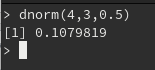
\includegraphics[scale=1]{praka1a}\\
  Diketahui:\\
  X = 4\\
  mean = 3\\
  sd = 0.5\\
  Pada soal a adalah mencari probabiliatas kumulatif x dengan rata-rata $\lambda$
  Atau P(X = x), sehingga kita gunakan perintah dnorm, format dari perintah dnorm adalah seperti berikut\\
  \texttt{>dnorm(x, mean, sd)\\}
  Jadi untuk soal ini perintahnya adalah\\
  \texttt{dnorm(4,3,0.5)}\\
  Dari output di atas diketahui bahwa $P(X = 4) = 0,10798$
  \item $P (X < 3,5)$
\end{enumerate}

\end{enumerate}
\end{document}
